\section{Numerical realization of the bisection}
\label{sec:numer-real-mount}

The procedure described in \ref{sec:bisection} can be easily realized
by solving the PDE \eqref{eq:en_flow} numerically. For $H_+$, we start
by choosing $g_+$ to be
\begin{align}
  \label{eq:98}
  g_+(\psi)=\sin\psi.
\end{align}
Then, the proper $A^*$ is found by bisection between the blow-up and
the convergence to $0$. As the bisection cannot yield an exact value
of $A^*$ (due to the finite machine precision) we are not able to
reach precisely the saddle point. Rather, as we are starting a bit off
the border between attractors, the solution slides along it reaching
the neighbourhood of $f_2$ along its stable direction, it stays there
for some time but then starts to move away, slowly decaying along the
unstable direction to finally either fall into $0$ or blow up. The
smaller the numerical error of $A^*$ the closer we get to the border
and the longer solutions stays near $f_2$.\\

From the numerical solutions to PDE \eqref{eq:en_flow} we can read off
the quantities involved in approaching and leaving the neighbourhood
of $f_2$. These are the first two modes of $f_2$ along with their
respective eigenvalues as presented in \eqref{eq:69}. To obtain the
eigenvalues $\lb{2}{0,2}$ we use the function $\partial_t\partial_\psi
f\big|_{\psi=0}$ which, while in a close neighbourhood of $f_2$ is
\begin{align}
  \label{eq:99}
  \partial_t\partial_\psi
  f\big|_{\psi=0}=C_0e^{-\lb{2}{0}t}+C_2e^{-\lb{2}{2}t}.
\end{align}
After obtaining the data points from numerically solving PDE
\eqref{eq:en_flow}, we fit \eqref{eq:99} with $C_{0,2}$ and
$\lb{2}{0,2}$ as free parameters.  $C_{0,2}$ depend on the
normalization of the unknown functions $v_{0,2}$ and their numerical
values are insignificant to us. The same relation can be used to
determine $\lb{3}{1,3}$ while close to $f_3$ by
\begin{align}
  \label{eq:101}
  \partial_t\partial_\psi
  f\big|_{\psi=0}=C_0e^{-\lb{3}{1}t}+C_2e^{-\lb{3}{3}t},
\end{align}
and similarly for $f_{0,1}$
\begin{align}
  \label{eq:100}
  \partial_t\partial_\psi f\big|_{\psi=0}&=D_{0}e^{-\lb{0}{0}} \\
  \label{eq:102}
  \partial_t\partial_\psi f\big|_{\psi=0}&=D_{1}e^{-\lb{1}{0}}.
\end{align}

The results from fitting to \eqref{eq:99} and \eqref{eq:101} compared
to numerically solving \eqref{eq:42} are shown in the table
\ref{tab:Lambda_comp}.

\begin{table}[h]
  \centering
  \begin{tabular}{| c | c | c | c |}\hline
    $\lb{n}{m}$ & Heat flow & Eigenproblem \\\hline
    $\lb{0}{0}$ & 2.9670        & 3            \\\hline
    $\lb{1}{1}$ & 3.9963        & 4            \\\hline
    $\lb{2}{0}$ & -2.8924       & -2.8926      \\\hline
    $\lb{2}{2}$ & 4.5899        & 4.5911       \\\hline
    $\lb{3}{1}$ & -10.5946      & -10.6650     \\\hline
    $\lb{3}{3}$ & 4.4004        & 4.3942       \\\hline
  \end{tabular}
  \caption{Comparison of the eigenvalues calculated by solving
    \eqref{eq:en_flow} and by solving \eqref{eq:42} for $k=3$. The
    values from solving eigenproblem for $n=0,1$ are exact by
    \eqref{eq:61} and \eqref{eq:68}.}
  \label{tab:Lambda_comp}
\end{table}


\section{Details of numerical calculations}
\label{sec:deta-numer-calc}

Both, the eigenproblem and the heat flow have been simulated using
the programs written in ANSI C and using double precision
arithmetic. The GSL library provided the set of standard time marching
procedures using Runge-Kutta algorithms \cite{Galassi}.\\

ODE \eqref{eq:f_psi_EL} have been solved by shooting from
$(\psi,f)=(0,0)$ to the saddle points $(\pi,0)$ and $(\pi,\pi)$.
Eigenproblem has been solved parallel to the ODE \eqref{eq:f_psi_EL}
and eigenvalues have been obtained by the shooting method as well. In
both problems we have used the series approximation to start near
$(0,0)$ but not at $(0,0)$, as $(0,0)$ is a saddle point.\\

The PDE \eqref{eq:33} have been solved using the methods of lines with
the derivatives on r.h.s. of \eqref{eq:33} approximated by the three
point stencils (order $2$ for the first derivative, order $1$ for the
second derivative). Stencils were symmetric inside the grid and
asymmetric on both of its edges. The time marching was run by the
Runge-Kutta-Fehlberg (4,5) method from the GSL
library\cite{Galassi}. The details of the simulations giving rise to
the figures \ref{fig:snapshot_f2}--\ref{fig:Stages_f3} are given in
table \ref{tab:num_details}.



\begin{table}[ht]
  \centering
  \begin{tabular}{|c|c|c|}\hline
    Grid points       & 400                     & 400                     \\\hline
    Domain            & $[0,\pi/2]$             & $[0,\pi]$               \\\hline
    Initial data      & $\psi+B\sin(2\psi)$     & $A\sin(\psi)$           \\\hline
    Critical value    & $B=1.24571310318894035$ & $A=2.10669393489537526$ \\\hline
    Bisection error   & $B^*=B\pm10^{-15}\%$    & $A^*=A\pm10^{-15}\%$    \\\hline
    Stepping function & \verb|rkf45|            & \verb|rkf45|            \\\hline
  \end{tabular}
  \caption{Detailed parameters of numerical simulations.}
  \label{tab:num_details}
\end{table}


\begin{figure}[h]
  \centering \advance\leftskip-3cm
  % GNUPLOT: LaTeX picture with Postscript
\begingroup
  \makeatletter
  \providecommand\color[2][]{%
    \GenericError{(gnuplot) \space\space\space\@spaces}{%
      Package color not loaded in conjunction with
      terminal option `colourtext'%
    }{See the gnuplot documentation for explanation.%
    }{Either use 'blacktext' in gnuplot or load the package
      color.sty in LaTeX.}%
    \renewcommand\color[2][]{}%
  }%
  \providecommand\includegraphics[2][]{%
    \GenericError{(gnuplot) \space\space\space\@spaces}{%
      Package graphicx or graphics not loaded%
    }{See the gnuplot documentation for explanation.%
    }{The gnuplot epslatex terminal needs graphicx.sty or graphics.sty.}%
    \renewcommand\includegraphics[2][]{}%
  }%
  \providecommand\rotatebox[2]{#2}%
  \@ifundefined{ifGPcolor}{%
    \newif\ifGPcolor
    \GPcolortrue
  }{}%
  \@ifundefined{ifGPblacktext}{%
    \newif\ifGPblacktext
    \GPblacktexttrue
  }{}%
  % define a \g@addto@macro without @ in the name:
  \let\gplgaddtomacro\g@addto@macro
  % define empty templates for all commands taking text:
  \gdef\gplbacktext{}%
  \gdef\gplfronttext{}%
  \makeatother
  \ifGPblacktext
    % no textcolor at all
    \def\colorrgb#1{}%
    \def\colorgray#1{}%
  \else
    % gray or color?
    \ifGPcolor
      \def\colorrgb#1{\color[rgb]{#1}}%
      \def\colorgray#1{\color[gray]{#1}}%
      \expandafter\def\csname LTw\endcsname{\color{white}}%
      \expandafter\def\csname LTb\endcsname{\color{black}}%
      \expandafter\def\csname LTa\endcsname{\color{black}}%
      \expandafter\def\csname LT0\endcsname{\color[rgb]{1,0,0}}%
      \expandafter\def\csname LT1\endcsname{\color[rgb]{0,1,0}}%
      \expandafter\def\csname LT2\endcsname{\color[rgb]{0,0,1}}%
      \expandafter\def\csname LT3\endcsname{\color[rgb]{1,0,1}}%
      \expandafter\def\csname LT4\endcsname{\color[rgb]{0,1,1}}%
      \expandafter\def\csname LT5\endcsname{\color[rgb]{1,1,0}}%
      \expandafter\def\csname LT6\endcsname{\color[rgb]{0,0,0}}%
      \expandafter\def\csname LT7\endcsname{\color[rgb]{1,0.3,0}}%
      \expandafter\def\csname LT8\endcsname{\color[rgb]{0.5,0.5,0.5}}%
    \else
      % gray
      \def\colorrgb#1{\color{black}}%
      \def\colorgray#1{\color[gray]{#1}}%
      \expandafter\def\csname LTw\endcsname{\color{white}}%
      \expandafter\def\csname LTb\endcsname{\color{black}}%
      \expandafter\def\csname LTa\endcsname{\color{black}}%
      \expandafter\def\csname LT0\endcsname{\color{black}}%
      \expandafter\def\csname LT1\endcsname{\color{black}}%
      \expandafter\def\csname LT2\endcsname{\color{black}}%
      \expandafter\def\csname LT3\endcsname{\color{black}}%
      \expandafter\def\csname LT4\endcsname{\color{black}}%
      \expandafter\def\csname LT5\endcsname{\color{black}}%
      \expandafter\def\csname LT6\endcsname{\color{black}}%
      \expandafter\def\csname LT7\endcsname{\color{black}}%
      \expandafter\def\csname LT8\endcsname{\color{black}}%
    \fi
  \fi
  \setlength{\unitlength}{0.0500bp}%
  \begin{picture}(10080.00,10080.00)%
    \gplgaddtomacro\gplbacktext{%
      \csname LTb\endcsname%
      \put(1814,6579){\makebox(0,0){\strut{}$t=0.0$}}%
    }%
    \gplgaddtomacro\gplfronttext{%
    }%
    \gplgaddtomacro\gplbacktext{%
      \csname LTb\endcsname%
      \put(2488,8534){\makebox(0,0)[r]{\strut{}$\pi/2$}}%
      \csname LTb\endcsname%
      \put(3157,7777){\makebox(0,0){\strut{}$\pi/2$}}%
    }%
    \gplgaddtomacro\gplfronttext{%
    }%
    \gplgaddtomacro\gplbacktext{%
      \csname LTb\endcsname%
      \put(4502,6579){\makebox(0,0){\strut{}$t=1.4$}}%
    }%
    \gplgaddtomacro\gplfronttext{%
    }%
    \gplgaddtomacro\gplbacktext{%
    }%
    \gplgaddtomacro\gplfronttext{%
    }%
    \gplgaddtomacro\gplbacktext{%
      \csname LTb\endcsname%
      \put(7189,6579){\makebox(0,0){\strut{}$t=2.9$}}%
    }%
    \gplgaddtomacro\gplfronttext{%
    }%
    \gplgaddtomacro\gplbacktext{%
    }%
    \gplgaddtomacro\gplfronttext{%
    }%
    \gplgaddtomacro\gplbacktext{%
      \csname LTb\endcsname%
      \put(1814,3891){\makebox(0,0){\strut{}$t=4.3$}}%
    }%
    \gplgaddtomacro\gplfronttext{%
    }%
    \gplgaddtomacro\gplbacktext{%
    }%
    \gplgaddtomacro\gplfronttext{%
    }%
    \gplgaddtomacro\gplbacktext{%
      \csname LTb\endcsname%
      \put(4502,3891){\makebox(0,0){\strut{}$t=5.8$}}%
    }%
    \gplgaddtomacro\gplfronttext{%
    }%
    \gplgaddtomacro\gplbacktext{%
    }%
    \gplgaddtomacro\gplfronttext{%
    }%
    \gplgaddtomacro\gplbacktext{%
      \csname LTb\endcsname%
      \put(7189,3891){\makebox(0,0){\strut{}$t=7.2$}}%
    }%
    \gplgaddtomacro\gplfronttext{%
    }%
    \gplgaddtomacro\gplbacktext{%
    }%
    \gplgaddtomacro\gplfronttext{%
    }%
    \gplgaddtomacro\gplbacktext{%
      \csname LTb\endcsname%
      \put(876,1008){\makebox(0,0)[r]{\strut{}$10^{-2}$}}%
      \put(876,1680){\makebox(0,0)[r]{\strut{}$10^{-1}$}}%
      \put(876,2351){\makebox(0,0)[r]{\strut{}$10^{0}$}}%
      \put(876,3023){\makebox(0,0)[r]{\strut{}$10^{1}$}}%
      \put(876,3695){\makebox(0,0)[r]{\strut{}$10^{2}$}}%
      \put(1008,788){\makebox(0,0){\strut{}$0$}}%
      \put(2352,788){\makebox(0,0){\strut{}$\pi/4$}}%
      \put(3696,788){\makebox(0,0){\strut{}$\pi/2$}}%
      \put(1008,788){\makebox(0,0){\strut{}}}%
      \put(2352,788){\makebox(0,0){\strut{}}}%
      \put(3696,788){\makebox(0,0){\strut{}}}%
      \put(-17,2351){\rotatebox{90}{\makebox(0,0){\strut{}$|\partial_t f(t,\psi)|$}}}%
      \put(2352,458){\makebox(0,0){\strut{}$\psi$}}%
      \put(1814,1203){\makebox(0,0){\strut{}$t=8.7$}}%
    }%
    \gplgaddtomacro\gplfronttext{%
    }%
    \gplgaddtomacro\gplbacktext{%
    }%
    \gplgaddtomacro\gplfronttext{%
    }%
    \gplgaddtomacro\gplbacktext{%
      \csname LTb\endcsname%
      \put(4502,1203){\makebox(0,0){\strut{}$t=10.$}}%
    }%
    \gplgaddtomacro\gplfronttext{%
    }%
    \gplgaddtomacro\gplbacktext{%
    }%
    \gplgaddtomacro\gplfronttext{%
    }%
    \gplgaddtomacro\gplbacktext{%
      \csname LTb\endcsname%
      \put(7189,1203){\makebox(0,0){\strut{}$t=11.$}}%
      \put(8265,2083){\makebox(0,0)[l]{\strut{}$\vn{0}{2}$}}%
      \put(7996,1545){\makebox(0,0)[l]{\strut{}$\vn{2}{2}$}}%
    }%
    \gplgaddtomacro\gplfronttext{%
    }%
    \gplgaddtomacro\gplbacktext{%
    }%
    \gplgaddtomacro\gplfronttext{%
    }%
    \gplbacktext
    \put(0,0){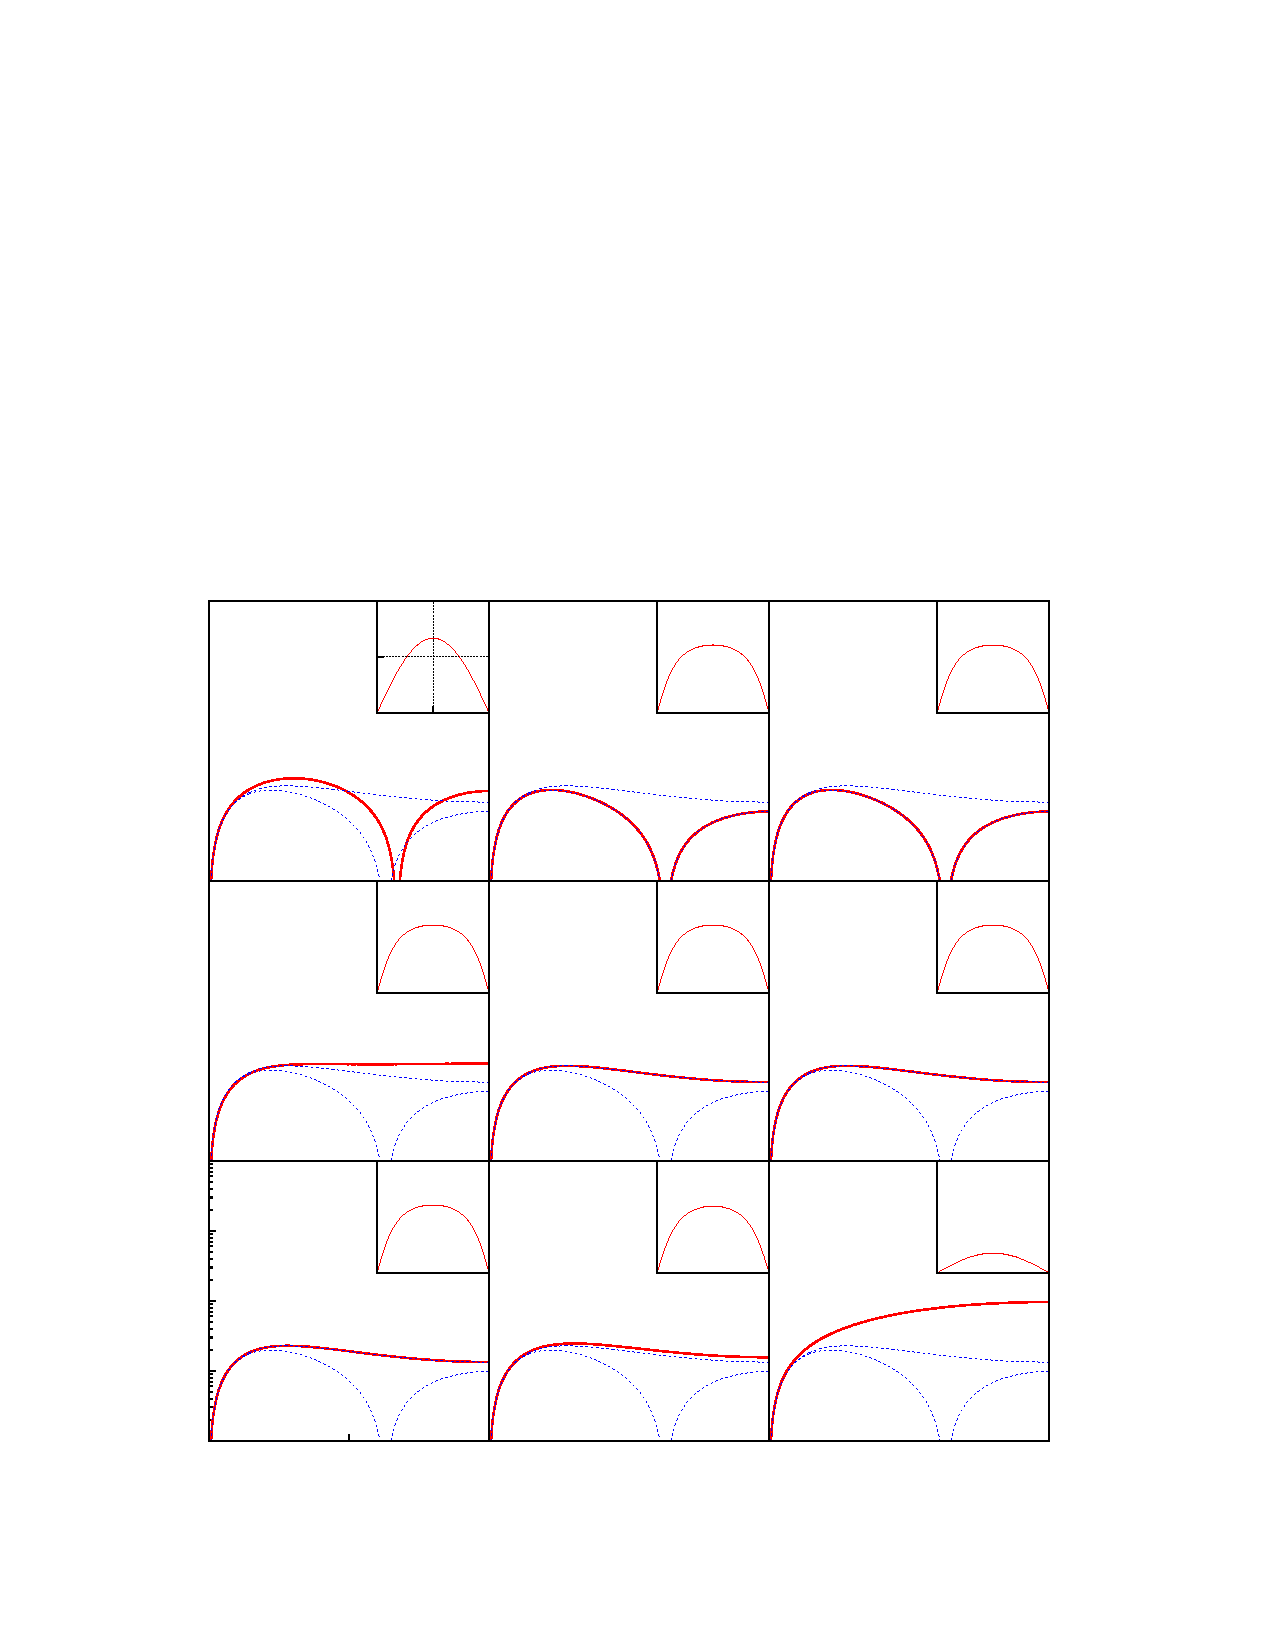
\includegraphics{graphics/snapshot_f2}}%
    \gplfronttext
  \end{picture}%
\endgroup

  \caption{Sequence of snapshots of numerical solutions to the heat
    flow with initial data $g_+(\psi)=A\cdot \sin(\psi)$ with $A$ as
    in \ref{tab:num_details}. Each snapshot depicts $\lvert \partial_t
    f\rvert$ (red line, larger plot) normalized so that
    $\lvert \partial_t\partial_\psi f(t,0)\rvert=1$ along with the
    plot of $f(t)$ (the plot in the upper right corner). For
    comparison the first two modes of $f_2$ (blue dashed lines),
    normalized to $v_{0,2}^{(2)\prime}(0)=1$ have been also
    depicted. The evolution can now be divided into the following
    stages: ($t=0.0$) non-linear approach to $f_2$, ($t=1.4-2.9$)
    linear convergence to $f_2$ along $\vn{2}{2}$, ($t=4.3-10.$)
    linear divergence along $\vn{0}{2}$, ($t=3.5$) non-linear approach
    to ground state $f_0$, ($t\ge4$) linear convergence to $f_1$ along
    $\vn{1}{1}$.}\label{fig:snapshot_f2}
\end{figure}

\begin{figure}[h]
  \centering \advance\leftskip-3cm
  % GNUPLOT: LaTeX picture with Postscript
\begingroup
  \makeatletter
  \providecommand\color[2][]{%
    \GenericError{(gnuplot) \space\space\space\@spaces}{%
      Package color not loaded in conjunction with
      terminal option `colourtext'%
    }{See the gnuplot documentation for explanation.%
    }{Either use 'blacktext' in gnuplot or load the package
      color.sty in LaTeX.}%
    \renewcommand\color[2][]{}%
  }%
  \providecommand\includegraphics[2][]{%
    \GenericError{(gnuplot) \space\space\space\@spaces}{%
      Package graphicx or graphics not loaded%
    }{See the gnuplot documentation for explanation.%
    }{The gnuplot epslatex terminal needs graphicx.sty or graphics.sty.}%
    \renewcommand\includegraphics[2][]{}%
  }%
  \providecommand\rotatebox[2]{#2}%
  \@ifundefined{ifGPcolor}{%
    \newif\ifGPcolor
    \GPcolortrue
  }{}%
  \@ifundefined{ifGPblacktext}{%
    \newif\ifGPblacktext
    \GPblacktexttrue
  }{}%
  % define a \g@addto@macro without @ in the name:
  \let\gplgaddtomacro\g@addto@macro
  % define empty templates for all commands taking text:
  \gdef\gplbacktext{}%
  \gdef\gplfronttext{}%
  \makeatother
  \ifGPblacktext
    % no textcolor at all
    \def\colorrgb#1{}%
    \def\colorgray#1{}%
  \else
    % gray or color?
    \ifGPcolor
      \def\colorrgb#1{\color[rgb]{#1}}%
      \def\colorgray#1{\color[gray]{#1}}%
      \expandafter\def\csname LTw\endcsname{\color{white}}%
      \expandafter\def\csname LTb\endcsname{\color{black}}%
      \expandafter\def\csname LTa\endcsname{\color{black}}%
      \expandafter\def\csname LT0\endcsname{\color[rgb]{1,0,0}}%
      \expandafter\def\csname LT1\endcsname{\color[rgb]{0,1,0}}%
      \expandafter\def\csname LT2\endcsname{\color[rgb]{0,0,1}}%
      \expandafter\def\csname LT3\endcsname{\color[rgb]{1,0,1}}%
      \expandafter\def\csname LT4\endcsname{\color[rgb]{0,1,1}}%
      \expandafter\def\csname LT5\endcsname{\color[rgb]{1,1,0}}%
      \expandafter\def\csname LT6\endcsname{\color[rgb]{0,0,0}}%
      \expandafter\def\csname LT7\endcsname{\color[rgb]{1,0.3,0}}%
      \expandafter\def\csname LT8\endcsname{\color[rgb]{0.5,0.5,0.5}}%
    \else
      % gray
      \def\colorrgb#1{\color{black}}%
      \def\colorgray#1{\color[gray]{#1}}%
      \expandafter\def\csname LTw\endcsname{\color{white}}%
      \expandafter\def\csname LTb\endcsname{\color{black}}%
      \expandafter\def\csname LTa\endcsname{\color{black}}%
      \expandafter\def\csname LT0\endcsname{\color{black}}%
      \expandafter\def\csname LT1\endcsname{\color{black}}%
      \expandafter\def\csname LT2\endcsname{\color{black}}%
      \expandafter\def\csname LT3\endcsname{\color{black}}%
      \expandafter\def\csname LT4\endcsname{\color{black}}%
      \expandafter\def\csname LT5\endcsname{\color{black}}%
      \expandafter\def\csname LT6\endcsname{\color{black}}%
      \expandafter\def\csname LT7\endcsname{\color{black}}%
      \expandafter\def\csname LT8\endcsname{\color{black}}%
    \fi
  \fi
  \setlength{\unitlength}{0.0500bp}%
  \begin{picture}(10080.00,10080.00)%
    \gplgaddtomacro\gplbacktext{%
      \csname LTb\endcsname%
      \put(2889,6579){\makebox(0,0){\strut{}$t=0.0$}}%
    }%
    \gplgaddtomacro\gplfronttext{%
    }%
    \gplgaddtomacro\gplbacktext{%
      \csname LTb\endcsname%
      \put(2488,8534){\makebox(0,0)[r]{\strut{}$\pi/2$}}%
      \csname LTb\endcsname%
      \put(3157,7777){\makebox(0,0){\strut{}$\pi/2$}}%
    }%
    \gplgaddtomacro\gplfronttext{%
    }%
    \gplgaddtomacro\gplbacktext{%
      \csname LTb\endcsname%
      \put(5577,6579){\makebox(0,0){\strut{}$t=0.5$}}%
    }%
    \gplgaddtomacro\gplfronttext{%
    }%
    \gplgaddtomacro\gplbacktext{%
    }%
    \gplgaddtomacro\gplfronttext{%
    }%
    \gplgaddtomacro\gplbacktext{%
      \csname LTb\endcsname%
      \put(8264,6579){\makebox(0,0){\strut{}$t=1.0$}}%
    }%
    \gplgaddtomacro\gplfronttext{%
    }%
    \gplgaddtomacro\gplbacktext{%
    }%
    \gplgaddtomacro\gplfronttext{%
    }%
    \gplgaddtomacro\gplbacktext{%
      \csname LTb\endcsname%
      \put(2889,3891){\makebox(0,0){\strut{}$t=1.5$}}%
    }%
    \gplgaddtomacro\gplfronttext{%
    }%
    \gplgaddtomacro\gplbacktext{%
    }%
    \gplgaddtomacro\gplfronttext{%
    }%
    \gplgaddtomacro\gplbacktext{%
      \csname LTb\endcsname%
      \put(5577,3891){\makebox(0,0){\strut{}$t=2.0$}}%
    }%
    \gplgaddtomacro\gplfronttext{%
    }%
    \gplgaddtomacro\gplbacktext{%
    }%
    \gplgaddtomacro\gplfronttext{%
    }%
    \gplgaddtomacro\gplbacktext{%
      \csname LTb\endcsname%
      \put(8264,3891){\makebox(0,0){\strut{}$t=2.5$}}%
    }%
    \gplgaddtomacro\gplfronttext{%
    }%
    \gplgaddtomacro\gplbacktext{%
    }%
    \gplgaddtomacro\gplfronttext{%
    }%
    \gplgaddtomacro\gplbacktext{%
      \csname LTb\endcsname%
      \put(876,1008){\makebox(0,0)[r]{\strut{}$10^{-2}$}}%
      \put(876,1680){\makebox(0,0)[r]{\strut{}$10^{-1}$}}%
      \put(876,2351){\makebox(0,0)[r]{\strut{}$10^{0}$}}%
      \put(876,3023){\makebox(0,0)[r]{\strut{}$10^{1}$}}%
      \put(876,3695){\makebox(0,0)[r]{\strut{}$10^{2}$}}%
      \put(1008,788){\makebox(0,0){\strut{}$0$}}%
      \put(2352,788){\makebox(0,0){\strut{}$\pi/4$}}%
      \put(3696,788){\makebox(0,0){\strut{}$\pi/2$}}%
      \put(1008,788){\makebox(0,0){\strut{}}}%
      \put(2352,788){\makebox(0,0){\strut{}}}%
      \put(3696,788){\makebox(0,0){\strut{}}}%
      \put(-17,2351){\rotatebox{90}{\makebox(0,0){\strut{}$|\partial_t f(t,\psi)|$}}}%
      \put(2352,458){\makebox(0,0){\strut{}$\psi$}}%
      \put(2889,1203){\makebox(0,0){\strut{}$t=3.0$}}%
    }%
    \gplgaddtomacro\gplfronttext{%
    }%
    \gplgaddtomacro\gplbacktext{%
    }%
    \gplgaddtomacro\gplfronttext{%
    }%
    \gplgaddtomacro\gplbacktext{%
      \csname LTb\endcsname%
      \put(5577,1203){\makebox(0,0){\strut{}$t=3.5$}}%
    }%
    \gplgaddtomacro\gplfronttext{%
    }%
    \gplgaddtomacro\gplbacktext{%
    }%
    \gplgaddtomacro\gplfronttext{%
    }%
    \gplgaddtomacro\gplbacktext{%
      \csname LTb\endcsname%
      \put(8264,1203){\makebox(0,0){\strut{}$t=4.0$}}%
      \put(7190,3158){\makebox(0,0)[l]{\strut{}$\vn{1}{3}$}}%
      \put(6652,2674){\makebox(0,0)[l]{\strut{}$\vn{3}{3}$}}%
    }%
    \gplgaddtomacro\gplfronttext{%
    }%
    \gplgaddtomacro\gplbacktext{%
    }%
    \gplgaddtomacro\gplfronttext{%
    }%
    \gplbacktext
    \put(0,0){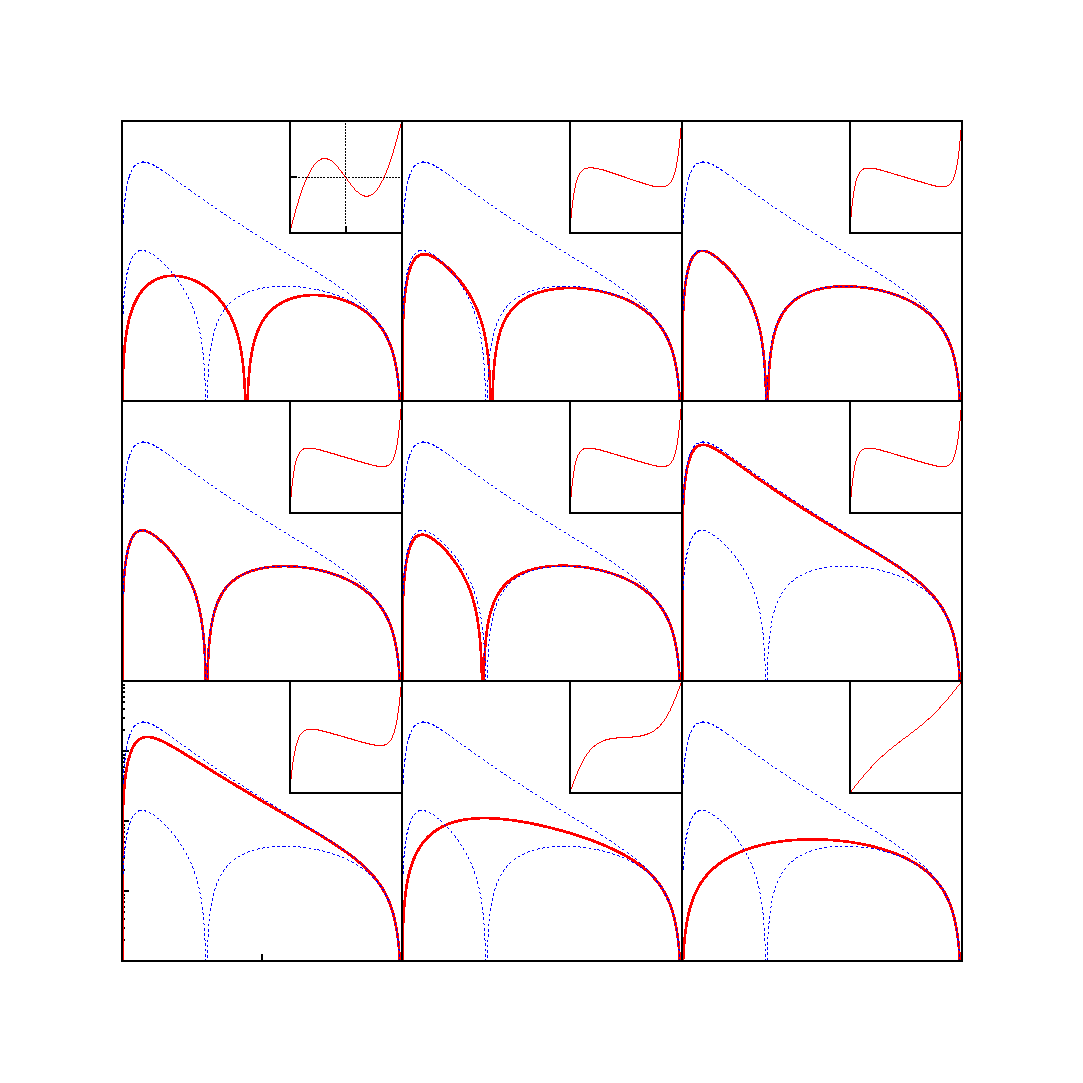
\includegraphics{graphics/snapshot_f3}}%
    \gplfronttext
  \end{picture}%
\endgroup

  \caption{Sequence of snapshots of numerical solutions to the heat
    flow with initial data $g_-(\psi)=\psi+B\cdot \sin(2\psi)$ with
    $B$ as in \ref{tab:num_details}. Each snapshot depicts
    $\lvert \partial_t f\rvert$ (red line, larger plot) normalized so
    that $\lvert \partial_t\partial_\psi f(t,\pi/2)\rvert=1$ along
    with the plot of $f(t)$ (the plot in the upper right corner). For
    comparison the first two modes of $f_3$ (blue dashed lines),
    normalized to $v_{1,3}^{(3)\prime}(\pi/2)=1$ have been also
    depicted. The evolution can now be divided into the following
    stages: ($t=0$) non-linear evolution, ($t=1.5-2$) linear
    convergence to $f_3$ along $\vn{3}{3}$, ($t=2.5-3.$) linear
    divergence along $\vn{1}{3}$, ($t=3.5$) non-linear approach to
    ground state $f_1$, ($t\ge4$) linear convergence to $f_1$ along
    $\vn{1}{1}$.}\label{fig:snapshot_f3}
\end{figure}

\begin{figure}[h]
  \centering \advance\leftskip-3cm
  % GNUPLOT: LaTeX picture with Postscript
\begingroup
  \makeatletter
  \providecommand\color[2][]{%
    \GenericError{(gnuplot) \space\space\space\@spaces}{%
      Package color not loaded in conjunction with
      terminal option `colourtext'%
    }{See the gnuplot documentation for explanation.%
    }{Either use 'blacktext' in gnuplot or load the package
      color.sty in LaTeX.}%
    \renewcommand\color[2][]{}%
  }%
  \providecommand\includegraphics[2][]{%
    \GenericError{(gnuplot) \space\space\space\@spaces}{%
      Package graphicx or graphics not loaded%
    }{See the gnuplot documentation for explanation.%
    }{The gnuplot epslatex terminal needs graphicx.sty or graphics.sty.}%
    \renewcommand\includegraphics[2][]{}%
  }%
  \providecommand\rotatebox[2]{#2}%
  \@ifundefined{ifGPcolor}{%
    \newif\ifGPcolor
    \GPcolorfalse
  }{}%
  \@ifundefined{ifGPblacktext}{%
    \newif\ifGPblacktext
    \GPblacktexttrue
  }{}%
  % define a \g@addto@macro without @ in the name:
  \let\gplgaddtomacro\g@addto@macro
  % define empty templates for all commands taking text:
  \gdef\gplbacktext{}%
  \gdef\gplfronttext{}%
  \makeatother
  \ifGPblacktext
    % no textcolor at all
    \def\colorrgb#1{}%
    \def\colorgray#1{}%
  \else
    % gray or color?
    \ifGPcolor
      \def\colorrgb#1{\color[rgb]{#1}}%
      \def\colorgray#1{\color[gray]{#1}}%
      \expandafter\def\csname LTw\endcsname{\color{white}}%
      \expandafter\def\csname LTb\endcsname{\color{black}}%
      \expandafter\def\csname LTa\endcsname{\color{black}}%
      \expandafter\def\csname LT0\endcsname{\color[rgb]{1,0,0}}%
      \expandafter\def\csname LT1\endcsname{\color[rgb]{0,1,0}}%
      \expandafter\def\csname LT2\endcsname{\color[rgb]{0,0,1}}%
      \expandafter\def\csname LT3\endcsname{\color[rgb]{1,0,1}}%
      \expandafter\def\csname LT4\endcsname{\color[rgb]{0,1,1}}%
      \expandafter\def\csname LT5\endcsname{\color[rgb]{1,1,0}}%
      \expandafter\def\csname LT6\endcsname{\color[rgb]{0,0,0}}%
      \expandafter\def\csname LT7\endcsname{\color[rgb]{1,0.3,0}}%
      \expandafter\def\csname LT8\endcsname{\color[rgb]{0.5,0.5,0.5}}%
    \else
      % gray
      \def\colorrgb#1{\color{black}}%
      \def\colorgray#1{\color[gray]{#1}}%
      \expandafter\def\csname LTw\endcsname{\color{white}}%
      \expandafter\def\csname LTb\endcsname{\color{black}}%
      \expandafter\def\csname LTa\endcsname{\color{black}}%
      \expandafter\def\csname LT0\endcsname{\color{black}}%
      \expandafter\def\csname LT1\endcsname{\color{black}}%
      \expandafter\def\csname LT2\endcsname{\color{black}}%
      \expandafter\def\csname LT3\endcsname{\color{black}}%
      \expandafter\def\csname LT4\endcsname{\color{black}}%
      \expandafter\def\csname LT5\endcsname{\color{black}}%
      \expandafter\def\csname LT6\endcsname{\color{black}}%
      \expandafter\def\csname LT7\endcsname{\color{black}}%
      \expandafter\def\csname LT8\endcsname{\color{black}}%
    \fi
  \fi
  \setlength{\unitlength}{0.0500bp}%
  \begin{picture}(10080.00,4320.00)%
    \gplgaddtomacro\gplbacktext{%
      \csname LTb\endcsname%
      \put(1650,704){\makebox(0,0)[r]{\strut{}$10^{-9}$}}%
      \put(1650,1039){\makebox(0,0)[r]{\strut{}$10^{-8}$}}%
      \put(1650,1374){\makebox(0,0)[r]{\strut{}$10^{-7}$}}%
      \put(1650,1710){\makebox(0,0)[r]{\strut{}$10^{-6}$}}%
      \put(1650,2045){\makebox(0,0)[r]{\strut{}$10^{-5}$}}%
      \put(1650,2380){\makebox(0,0)[r]{\strut{}$10^{-4}$}}%
      \put(1650,2715){\makebox(0,0)[r]{\strut{}$10^{-3}$}}%
      \put(1650,3050){\makebox(0,0)[r]{\strut{}$10^{-2}$}}%
      \put(1650,3386){\makebox(0,0)[r]{\strut{}$10^{-1}$}}%
      \put(1650,3721){\makebox(0,0)[r]{\strut{}$10^{0}$}}%
      \put(1650,4056){\makebox(0,0)[r]{\strut{}$10^{1}$}}%
      \put(1782,484){\makebox(0,0){\strut{} 0}}%
      \put(2778,484){\makebox(0,0){\strut{} 2}}%
      \put(3774,484){\makebox(0,0){\strut{} 4}}%
      \put(4770,484){\makebox(0,0){\strut{} 6}}%
      \put(5766,484){\makebox(0,0){\strut{} 8}}%
      \put(6762,484){\makebox(0,0){\strut{} 10}}%
      \put(7758,484){\makebox(0,0){\strut{} 12}}%
      \put(8754,484){\makebox(0,0){\strut{} 14}}%
      \put(9750,484){\makebox(0,0){\strut{} 16}}%
      \put(888,2380){\rotatebox{90}{\makebox(0,0){\strut{}$\lvert\partial_t\partial_\psi f(t,0)\rvert$}}}%
      \put(5766,154){\makebox(0,0){\strut{}$t$}}%
      \put(3774,3553){\makebox(0,0){\strut{}near $f_2$}}%
      \put(8754,3553){\makebox(0,0){\strut{}near $f_0$}}%
    }%
    \gplgaddtomacro\gplfronttext{%
    }%
    \gplbacktext
    \put(0,0){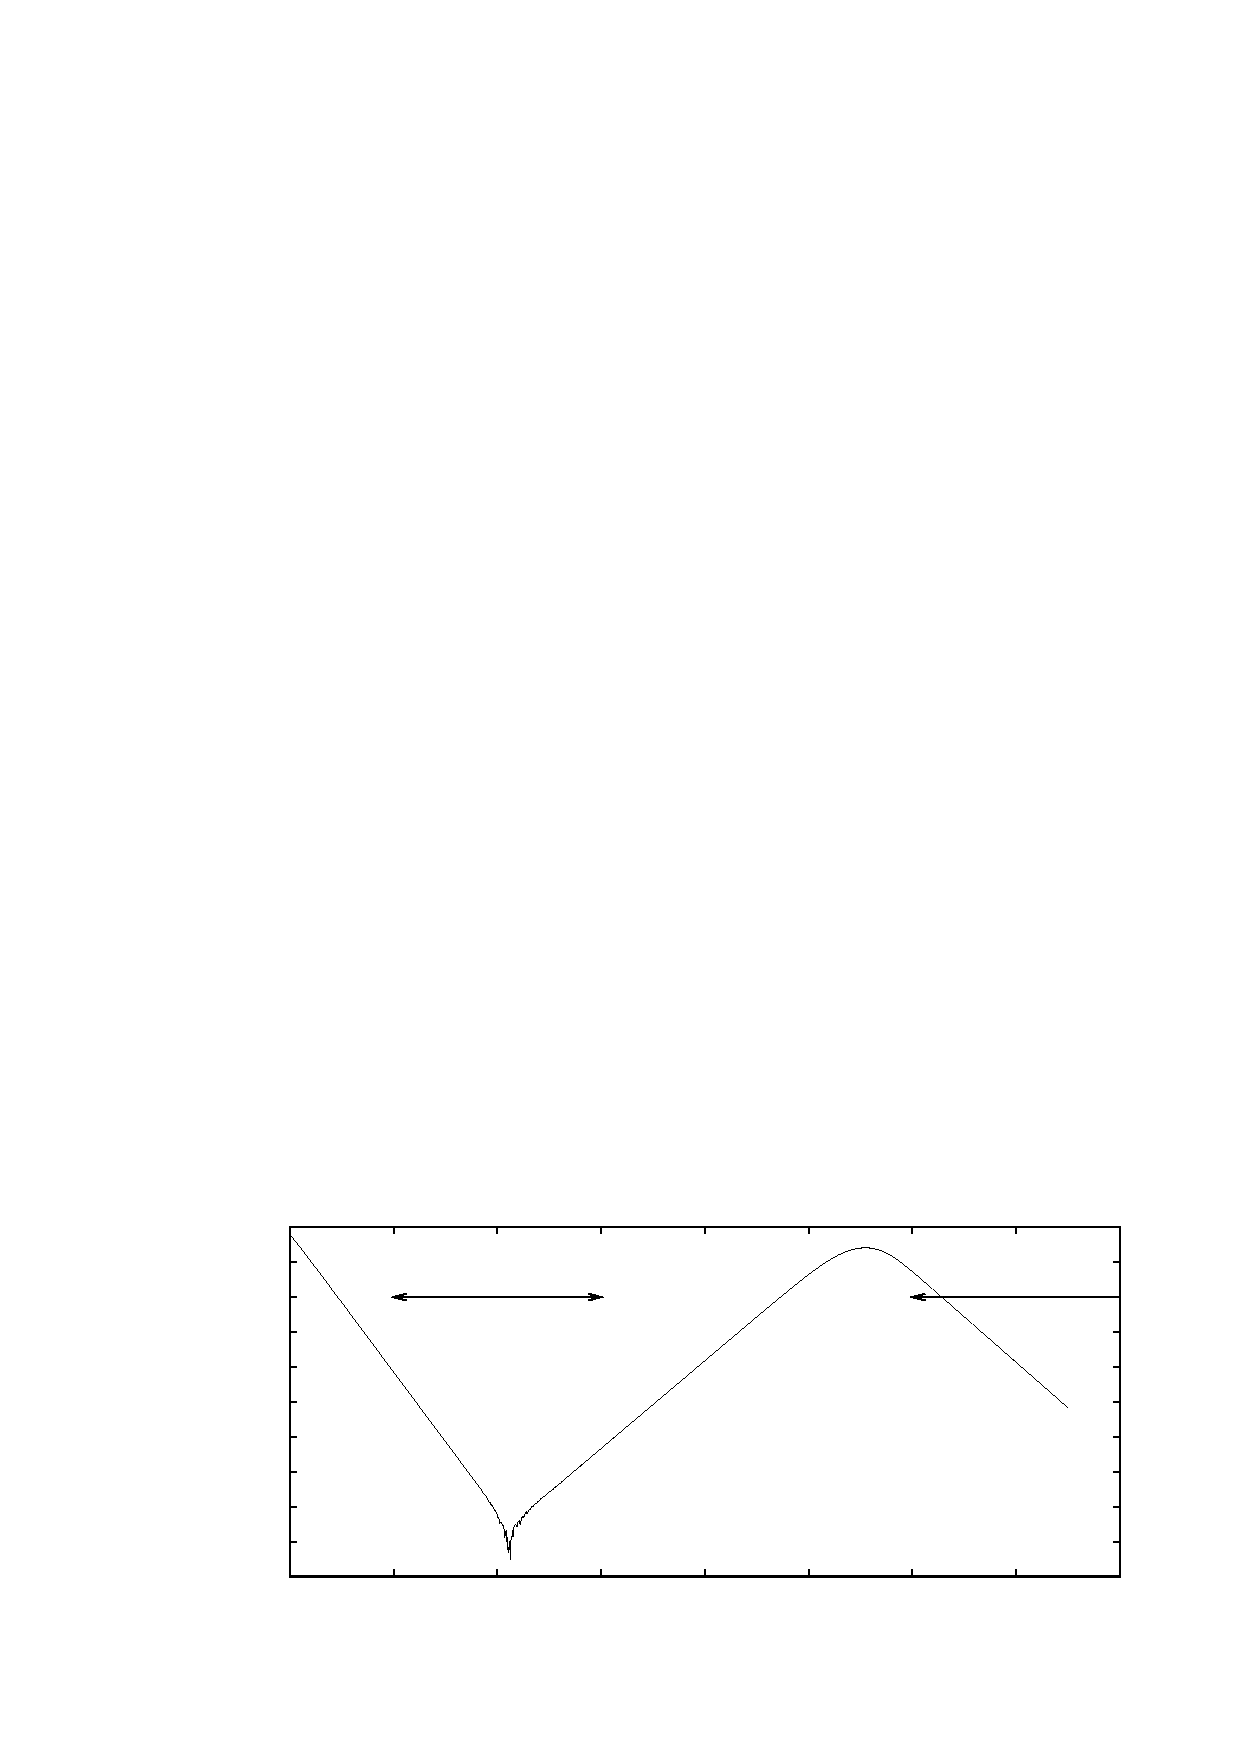
\includegraphics{./graphics/Gradient_flow_stages_f2}}%
    \gplfronttext
  \end{picture}%
\endgroup

  \caption{Stages of the heat flow evolution for symmetric initial
    data described in the caption of figure \ref{fig:snapshot_f2}.}
  \label{fig:Stages_f2}
\end{figure}

\begin{figure}[h]
  \centering \advance\leftskip-3cm
  % GNUPLOT: LaTeX picture with Postscript
\begingroup
  \makeatletter
  \providecommand\color[2][]{%
    \GenericError{(gnuplot) \space\space\space\@spaces}{%
      Package color not loaded in conjunction with
      terminal option `colourtext'%
    }{See the gnuplot documentation for explanation.%
    }{Either use 'blacktext' in gnuplot or load the package
      color.sty in LaTeX.}%
    \renewcommand\color[2][]{}%
  }%
  \providecommand\includegraphics[2][]{%
    \GenericError{(gnuplot) \space\space\space\@spaces}{%
      Package graphicx or graphics not loaded%
    }{See the gnuplot documentation for explanation.%
    }{The gnuplot epslatex terminal needs graphicx.sty or graphics.sty.}%
    \renewcommand\includegraphics[2][]{}%
  }%
  \providecommand\rotatebox[2]{#2}%
  \@ifundefined{ifGPcolor}{%
    \newif\ifGPcolor
    \GPcolorfalse
  }{}%
  \@ifundefined{ifGPblacktext}{%
    \newif\ifGPblacktext
    \GPblacktexttrue
  }{}%
  % define a \g@addto@macro without @ in the name:
  \let\gplgaddtomacro\g@addto@macro
  % define empty templates for all commands taking text:
  \gdef\gplbacktext{}%
  \gdef\gplfronttext{}%
  \makeatother
  \ifGPblacktext
    % no textcolor at all
    \def\colorrgb#1{}%
    \def\colorgray#1{}%
  \else
    % gray or color?
    \ifGPcolor
      \def\colorrgb#1{\color[rgb]{#1}}%
      \def\colorgray#1{\color[gray]{#1}}%
      \expandafter\def\csname LTw\endcsname{\color{white}}%
      \expandafter\def\csname LTb\endcsname{\color{black}}%
      \expandafter\def\csname LTa\endcsname{\color{black}}%
      \expandafter\def\csname LT0\endcsname{\color[rgb]{1,0,0}}%
      \expandafter\def\csname LT1\endcsname{\color[rgb]{0,1,0}}%
      \expandafter\def\csname LT2\endcsname{\color[rgb]{0,0,1}}%
      \expandafter\def\csname LT3\endcsname{\color[rgb]{1,0,1}}%
      \expandafter\def\csname LT4\endcsname{\color[rgb]{0,1,1}}%
      \expandafter\def\csname LT5\endcsname{\color[rgb]{1,1,0}}%
      \expandafter\def\csname LT6\endcsname{\color[rgb]{0,0,0}}%
      \expandafter\def\csname LT7\endcsname{\color[rgb]{1,0.3,0}}%
      \expandafter\def\csname LT8\endcsname{\color[rgb]{0.5,0.5,0.5}}%
    \else
      % gray
      \def\colorrgb#1{\color{black}}%
      \def\colorgray#1{\color[gray]{#1}}%
      \expandafter\def\csname LTw\endcsname{\color{white}}%
      \expandafter\def\csname LTb\endcsname{\color{black}}%
      \expandafter\def\csname LTa\endcsname{\color{black}}%
      \expandafter\def\csname LT0\endcsname{\color{black}}%
      \expandafter\def\csname LT1\endcsname{\color{black}}%
      \expandafter\def\csname LT2\endcsname{\color{black}}%
      \expandafter\def\csname LT3\endcsname{\color{black}}%
      \expandafter\def\csname LT4\endcsname{\color{black}}%
      \expandafter\def\csname LT5\endcsname{\color{black}}%
      \expandafter\def\csname LT6\endcsname{\color{black}}%
      \expandafter\def\csname LT7\endcsname{\color{black}}%
      \expandafter\def\csname LT8\endcsname{\color{black}}%
    \fi
  \fi
  \setlength{\unitlength}{0.0500bp}%
  \begin{picture}(10080.00,4320.00)%
    \gplgaddtomacro\gplbacktext{%
      \csname LTb\endcsname%
      \put(1650,704){\makebox(0,0)[r]{\strut{}$10^{-4}$}}%
      \put(1650,1263){\makebox(0,0)[r]{\strut{}$10^{-3}$}}%
      \put(1650,1821){\makebox(0,0)[r]{\strut{}$10^{-2}$}}%
      \put(1650,2380){\makebox(0,0)[r]{\strut{}$10^{-1}$}}%
      \put(1650,2939){\makebox(0,0)[r]{\strut{}$10^{0}$}}%
      \put(1650,3497){\makebox(0,0)[r]{\strut{}$10^{1}$}}%
      \put(1650,4056){\makebox(0,0)[r]{\strut{}$10^{2}$}}%
      \put(1782,484){\makebox(0,0){\strut{} 0}}%
      \put(3110,484){\makebox(0,0){\strut{} 1}}%
      \put(4438,484){\makebox(0,0){\strut{} 2}}%
      \put(5766,484){\makebox(0,0){\strut{} 3}}%
      \put(7094,484){\makebox(0,0){\strut{} 4}}%
      \put(8422,484){\makebox(0,0){\strut{} 5}}%
      \put(9750,484){\makebox(0,0){\strut{} 6}}%
      \put(888,2380){\rotatebox{90}{\makebox(0,0){\strut{}$\lvert\partial_t\partial_\psi f(t,0)\rvert$}}}%
      \put(5766,154){\makebox(0,0){\strut{}$t$}}%
      \put(4106,3553){\makebox(0,0){\strut{}near $f_3$}}%
      \put(8422,3553){\makebox(0,0){\strut{}near $f_1$}}%
    }%
    \gplgaddtomacro\gplfronttext{%
    }%
    \gplbacktext
    \put(0,0){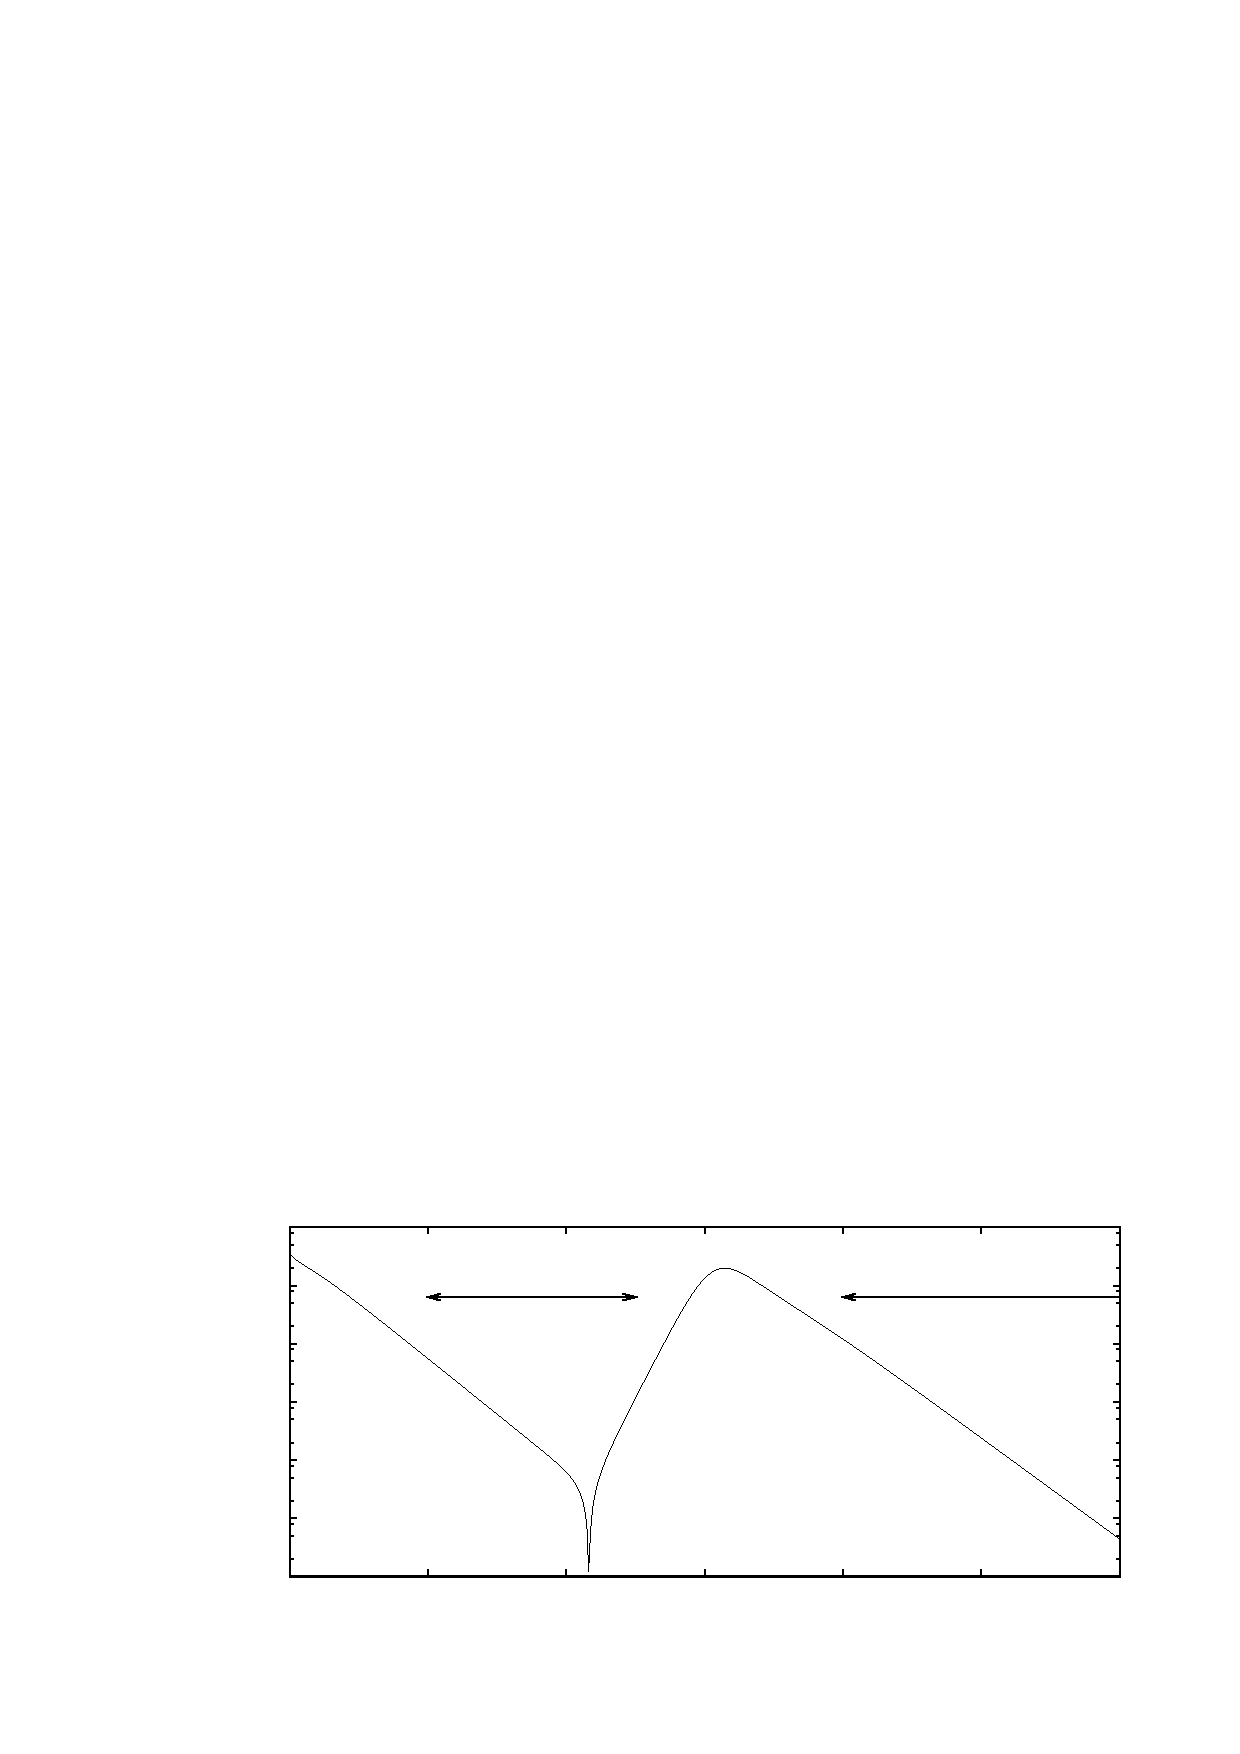
\includegraphics{./graphics/Gradient_flow_stages_f3}}%
    \gplfronttext
  \end{picture}%
\endgroup

  \caption{Stages of the heat flow evolution for antisymmetric
    initial data as described in the caption of figure \ref{fig:snapshot_f3}.}
  \label{fig:Stages_f3}
\end{figure}

%%% Local Variables:
%%% mode: latex
%%% TeX-master: "master"
%%% End:
